\documentclass[../main.tex]{subfiles}

\begin{document}
\section{Theory}\label{sec:theory}

\subsection{ODEs?}
\textcolor{red}{løst skrevet}
Newtons second law:
\begin{equation}\label{eq:newtons2}
    m\frac{d^2 x(t)}{dt^2} = -kx(t),
\end{equation} where $k$ is the force constant.

Rewrite equation (\ref{eq:newtons2}) using $x(t) = y^{(1)}(t)$ and $\frac{d y^{(1)}(t)}{dt} =  y^{(2)}(t)$ such that %$v(t) = y^{(2)}(t)$ such that  

\begin{equation}
    my^{(2)}(t) = -ky^{(1)}(t),
\end{equation}

Suppose we have an initial value for the function $y(t)$ given by $y_0 = y(t=t_0)$. Then, using the step size $h = \frac{b - a}{N}$ for the space $[a,b]$ with $N$ defining the number of steps needed to go from $a$ to $b$, we can move one step along $y(t)$ to find 
\begin{equation}\label{eq:y_1}
    y_1 = y(t_1 = t_0 + h)
\end{equation}
and so on. Depending on how well behaved the function is in the defined domain $[a, b]$, there might be a need for adaptive steps, however, in our case, a fixed step size will suffice. 

Next we will generalize equation (\ref{eq:y_1}), by writing in terms of steps, so that we get
\begin{equation}\label{eq:y_general}
    y_{i + 1} = y(t= t_i + h) = y(t_i) + h \Delta (t_i , y_i (t_i)) + O(h^{p + 1}), 
\end{equation}
where $O(h^{p + 1})$ is the truncation error. To determine $\Delta$, we can Taylor expand (\ref{eq:y_general}), which gives us 
\begin{equation}
    y_{i + 1} = y(t= t_i + h) = y(t_i) + h \left( y'(t_i) + ... + y^{p}(t_i) \frac{h^{p - 1}}{p!} \right) + O(h^{p + 1})
\end{equation}

\subsection{Conservation of angular momentum}
Kepler's 2\textsuperscript{nd} law, 

\begin{displayquote}
A radius vector joining any planet to the sun sweeps out equal areas in equal lengths of time \cite{Kepler2nd}, 
\end{displayquote} can be used to show conservation of angular momentum. We consider a small wedge of the orbit, as can be seen in \cref{fig:wedge}.

\begin{figure}[htb!]
    \centering
    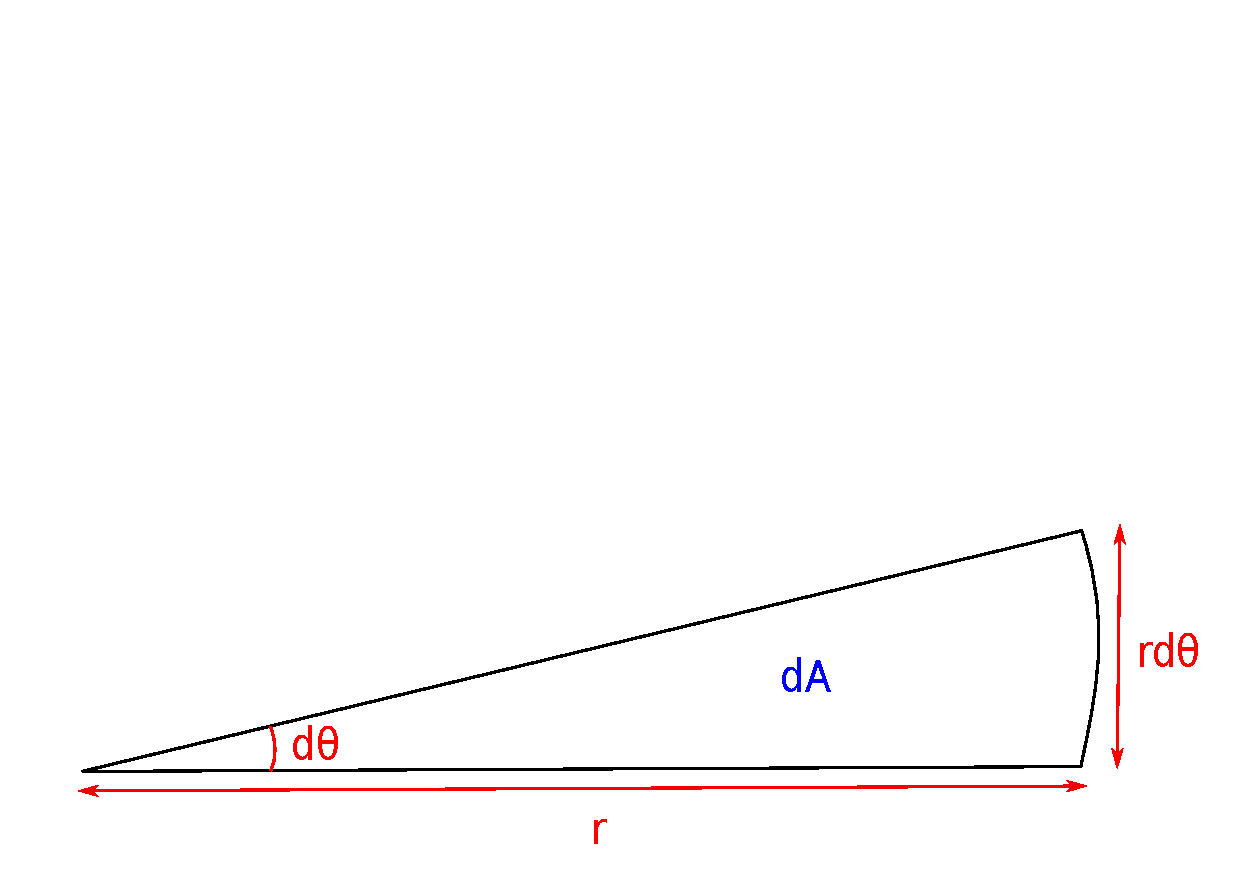
\includegraphics[trim=1cm 0.5cm 0.cm 8.5cm, clip,width=0.65\textwidth]{../figures/wedge_of_orbit.pdf}
    \caption{Wedge of Earths orbit.}
    \label{fig:wedge}
\end{figure}

The area of the wedge is given by
\begin{align*}
    dA = \frac{1}{2}rrd\theta.
\end{align*} The rate at which area is swept out in the orbit is then 

\begin{align*}
    \frac{dA}{dt}=\frac{1}{2}rr\frac{d\theta}{dt}=\frac{1}{2}rv_{\theta}=\textnormal{const.}
\end{align*} By inserting the definition of angular momentum, \ensuremath{L=mrv_{\theta}}, in the equation above, we get

\begin{align*}
    \frac{dA}{dt}=\frac{1}{2}\frac{L}{m}=\textnormal{const.}
\end{align*} Which shows that the angular momentum is conserved. 

\subsection{Escape velocity}

The kinetic energy of a body escaping the gravitational influence of another is given by \begin{equation}
    K = \frac{1}{2} m v_{e}^{2},
\end{equation} where $m$ is the mass of the the escaping body and $v_e$ is the escape velocity. 

If we then consider the force between two objects $F = G \frac{Mm}{r^2}$, then the work needed to move an infinitesimally small distance $dr$ is given by $dW = Fdr$. The work needed to move from a distance $r_0$ to a distance infinitely far away can so be found by 
\begin{equation}
W = \int_{r_0}^{\infty} F\, dr = \int_{r_0}^{\infty} G \frac{Mm}{r^2}\, dr = \left[ -\frac{GMm}{r}  \right]_{r_0}^{\infty} = \frac{GMm}{r_0},
\end{equation} were we define $M$ as the mass of the stationary object, $r$ as the distance between the two objects and $G$ as the gravitational constant.

To escape the gravitational influence of another body, the kinetic energy of the escaping body needs to be equal to the work required to move against the gravity of the stationary object from $r_0$ to $r = \infty$. That means that $K = W$, such that 
\begin{align}
    \frac{1}{2} m v_{e}^{2} = \frac{GMm}{r_0} \\
    v_{e}^{2} = \frac{2GM}{r_0} \\
    v_{e} = \sqrt{\frac{2GM}{r_0}},
\end{align}
which is the solution for the escape velocity. 
\iffalse
We are tasked with finding the initial velocity that will let a planet 1AU from the sun escape the sun. This initial velocity needs either to be equal to or bigger than the escape velocity to escape the sun, or it can be smaller, but then it would have to have an elliptical orbit that would speed it up enough to reach the escape velocity, if such a thing is possible. Either way, a velocity equal to the escape velocity at some point in orbit will guarantee an escape from the suns influence.
We need not consider the effects of the other planets on our escaping body, as the speed needed to escape the suns influence would be bigger than any contributions from the other planets. Ans should be about 40km/s
Can also be derived by setting K = U
\fi

\subsection{Generalization of Newton's gravitational law}
The modified gravitational force is given by 
\begin{align}
    \vec{F}=G\frac{M_{\odot} M_{\textnormal{\text{Earth}}}}{r^{\beta}}\vec{e}_r
\end{align} where \ensuremath{\vec{r}} is the position vector of the Earth relative to the sun and with \ensuremath{\beta \in [2,3]}. The corresponding potential can then be written

\begin{align}
    V = \frac{1}{\beta-1}\frac{M_{\odot} M_{\textnormal{\text{Earth}}}}{r^{\beta-1}}=\frac{1}{\alpha}\frac{GM_{\odot} M_{\text{Earth}}}{r^{\alpha}}
\end{align} \ensuremath{\alpha = \beta - 1}

The position vector of the Earth is given by

\begin{align*}
    \vec{r}=r(\cos\theta,\sin\theta).
\end{align*}

We define the Lagrangian of the system, given by

\begin{align*}
    \mathcal{L}=\frac{1}{2}M_{\text{Earth}}(\dot{r}^2+r^2\dot{\theta}^2)-\left(-\frac{1}{\alpha}\frac{GM_{\odot} M_{\text{Earth}}}{r^{\alpha}}\right).
\end{align*}

In \cref{sec:appendix_generalized_grav_law} we use conservation of total energy and angular momentum to show that the Lagrangian can be reduce to a one dimensional Lagrangian

\begin{align*}
    \mathcal{L}=\frac{1}{2}M_{\text{Earth}}\dot{r}^2-V_{\textnormal{eff}}(r),
\end{align*} where the effective potential is given by

\begin{align*}
    V_{\textnormal{eff}}(r)=\frac{1}{2}\frac{l^2}{M_{\text{Earth}}}\frac{1}{r^2}-\frac{1}{\beta-1}\frac{GM_{\odot}M_{\text{Earth}}}{r^{\alpha}}.
\end{align*} 

In \cref{sec:appendix_generalized_grav_law}, we also show that we must have \ensuremath{\beta<3} to have a stable equilibrium for Earths orbit. 

\subsection{Perihelion precession}

Adding a relativistic correction to the Newtonian gravitational force will change the orbit of the object, which in general is not closed without the inverse square form of the Newtonian gravitational force. For small corrections, this means that the object will follow an almost elliptical orbit, which can be thought of as an elliptical orbit that rotates slowly. We add a relativistic correction to the general Newtonian equation \cref{eq:} such that

\begin{align}
    F_G = \frac{G M_\odot M_{\textnormal{Mercury}}}{r^2} \left(1 + \frac{3l^2}{r^2 c^2} \right).
\end{align}

\subsection{Circular Orbits}

For the Earth-Sun system, a circular orbit means that the distance between the center of mass of the Sun and the Earth is equal to the constant radius $r_E$. Thus the Newtonian gravitational potential energy

\begin{align}
    E_p(r) = -\frac{G M_\odot M_E}{r}
\end{align}

will remain constant for a circular orbit. Since the overall sum of the kinetic energy and potential energy of a planetary body is conserved, conservation of the potential energy also implies conservation of kinetic energy.

The force between the Earth and the Sun is given by
\begin{equation}\label{eq:f_earth}
    F = M_E a = \frac{GM_\odot M_E}{r^2}.
\end{equation}
Using the fact that for a circular orbit $a = \frac{v^2}{r}$, we can rewrite (\ref{eq:f_earth}) to find
\begin{align}
    \frac{v^2}{r} &= \frac{GM_\odot}{r^2}\\
    v &= \sqrt{\frac{GM_\odot}{r}}.
\end{align}
\end{document}
